\documentclass[
	10pt,								% globale Schriftgröße
	parskip=half-,						% setzt Absatzabstand hoch
	paper=a4,							% Format
	english,ngerman,					% lädt Sprachpakete
	]{scrartcl}							% Dokumentenklasse

% //////////////////// Pakete laden ////////////////////
\usepackage{amsmath}			% MUSS vor fontspec geladen werden
\usepackage{mathtools}			% modifiziert amsmath
\usepackage{amssymb}			% mathematische symbole, für \ceckmarks
\usepackage{amsthm}				% für proof
\usepackage{mathrsfs}			% für \mathscr
\usepackage{latexsym}
\usepackage{marvosym}				% für Lightning

\usepackage{fontspec} 			% funktioniert nur mit den neueren Compilern z.B. XeLaTeX
\usepackage{microtype}			% für bessere Worttrennung
\usepackage[ngerman]{babel} 	% Spracheinstellung
\usepackage{lmodern}			% verändert verwendete Schriftart, damit sie weniger pixelig ist

\usepackage{verbatim}
\usepackage{listings}			% Für Quellcode

\usepackage{graphicx}
\usepackage{tabularx}			% für Tabellen mit gleicher Spaltenbreite und automatischen Umbrüchen
\usepackage{fullpage}
\usepackage{multirow}			% für multirow in tabulars
\usepackage{rotate}
\usepackage[cmyk,table]{xcolor} % um Farben zu benutzen, kann mehr als das Paket color
\usepackage[					% Verlinkungen
	colorlinks,					% farbige Schrift, statt farbiger Rahmen
	linktocpage,				% verlinkt im Abb.Verzeichnis Seitenzahl statt Bildunterschrift
	linkcolor=blue				% setzt Farbe der Links auf blau
	]{hyperref}					% nur für digitale Anwendungen, url = "http://www.example.com"
\usepackage{url}				% für Webadressen wie e-mail usw.: "\url{http://www.example.com}"

\usepackage{enumerate}			% für versch. Aufzählungezeichen wie z.B. a)
\usepackage{xspace}				% folgt ein Leerzeichen nach einem \Befehl, wird es nicht verschluckt.
\usepackage{cancel}				% für das Durchstreichen u.a. in Matheformeln mit \cancel
\usepackage{float}              % zum Forcieren der Position von figure-Umgebungen

% zum Zeichnen (u.a. von Graphen)
\usepackage{fp}
\usepackage{tikz}
\usetikzlibrary{tikzmark}			% für \tikzmark{toRemember}
\usetikzlibrary{positioning}	% verbesserte Positionierung der Knoten
\usetikzlibrary{automata}		% für Automaten (GTI)
\usetikzlibrary{arrows}
\usetikzlibrary{shapes}
\usetikzlibrary{decorations.pathmorphing}
\usetikzlibrary{decorations.pathreplacing}
\usetikzlibrary{decorations.shapes}
\usetikzlibrary{decorations.text}

% //////////////////// Syntaxhighlighting ////////////////////
\lstloadlanguages{Python, Haskell, [LaTeX]TeX, Java}
\lstset{
   basicstyle=\footnotesize\ttfamily,	% \scriptsize the size of the fonts that are used for the code
   backgroundcolor = \color{bgcolour},	% legt Farbe der Box fest
   breakatwhitespace=false,	% sets if automatic breaks should only happen at whitespace
   breaklines=true,			% sets automatic line breaking
   captionpos=t,				% sets the caption-position to bottom, t for top
   commentstyle=\color{codeblue}\ttfamily,% comment style
   frame=single,				% adds a frame around the code
   keepspaces=true,			% keeps spaces in text, useful for keeping indentation
							% of code (possibly needs columns=flexible)
   keywordstyle=\bfseries\ttfamily\color{codepurple},% keyword style
   numbers=left,				% where to put the line-numbers;
   							% possible values are (none, left, right)
   numberstyle=\tiny\color{codegreen},	% the style that is used for the line-numbers
   numbersep=5pt,			% how far the line-numbers are from the code
   stepnumber=1,				% nummeriert nur jede i-te Zeile
   showspaces=false,			% show spaces everywhere adding particular underscores;
							% it overrides 'showstringspaces'
   showstringspaces=false,	% underline spaces within strings only
   showtabs=false,			% show tabs within strings adding particular underscores
   flexiblecolumns=false,
   tabsize=1,				% the step between two line-numbers. If 1: each line will be numbered
   stringstyle=\color{orange}\ttfamily,	% string literal style
   numberblanklines=false,				% leere Zeilen werden nicht mitnummeriert
   xleftmargin=1.2em,					% Abstand zum linken Layoutrand
   xrightmargin=0.4em,					% Abstand zum rechten Layoutrand
   aboveskip=2ex, 
}

\lstdefinestyle{py}{
   language=Python,
}
\lstdefinestyle{hs}{
   language=Haskell,
}
\lstdefinestyle{tex}{
	language=[LaTeX]TeX,
	escapeinside={\%*}{*)},     % if you want to add LaTeX within your code
	texcsstyle=*\bfseries\color{blue},% hervorhebung der tex-Schlüsselwörter
	morekeywords={*,$,\{,\},\[,\],lstinputlisting,includegraphics,
	rowcolor,columncolor,listoffigures,lstlistoflistings,
	subsection,subsubsection,textcolor,tableofcontents,colorbox,
	fcolorbox,definecolor,cellcolor,url,linktocpage,subtitle,
	subject,maketitle,usetikzlibrary,node,path,addbibresource,
	printbibliography},% if you want to add more keywords to the set
     numbers=none,
     numbersep=0pt,
     xleftmargin=0.4em,
}

\lstdefinestyle{java}{
	language=Java,
	extendedchars=true,		% lets you use non-ASCII characters;
   						% for 8-bits encodings only, does not work with UTF-8
}

\lstdefinelanguage[x64]{Assembler}     % add a "x64" dialect of Assembler
   [x86masm]{Assembler} % based on the "x86masm" dialect
   % with these extra keywords:
   {morekeywords={CDQE,CQO,CMPSQ,CMPXCHG16B,JRCXZ,LODSQ,MOVSXD, %
                  POPFQ,PUSHFQ,SCASQ,STOSQ,IRETQ,RDTSCP,SWAPGS, %
                  rax,rdx,rcx,rbx,rsi,rdi,rsp,rbp, %
                  r8,r8d,r8w,r8b,r9,r9d,r9w,r9b}
}					% for 8-bits encodings only, does not work with UTF-8

\lstdefinestyle{c}{
	language=c,
	extendedchars=true,		% for 8-bits encodings only, does not work with UTF-8
}

% //////////////////// eigene Kommandos ////////////////////
\newcommand\FU{Freie Universität Berlin\xspace}% benötigt package xspace
\newcommand\gdw{g.\,d.\,w.\xspace}
\newcommand\oBdA{o.\,B.\,d.\,A.\xspace}
\newcommand{\Eu}{\texteuro}
\newcommand\N{\mathbb{N}\xspace}
\newcommand\Q{\mathbb{Q}\xspace}
\newcommand\R{\mathbb{R}\xspace}
\newcommand\Z{\mathbb{Z}\xspace}
\newcommand\ohneNull{\ensuremath{\backslash\lbrace 0\rbrace}}% \{0}
\let\dhALT\dh	% Schreibt Befehl \dh in \dhALT um
\renewcommand\dh{d.\,h.\xspace}	%renew überschreibt command \dh
\newcommand\Bolt{\;\text{\LARGE\raisebox{-0.3em}{\Lightning}\normalsize}\xspace}% Blitz
\newcommand\zz{\ensuremath{\raisebox{+0.25ex}{Z}% zu zeigen
			\kern-0.4em\raisebox{-0.25ex}{Z}%
			\;\xspace}}
\newcommand{\from}{\ensuremath{\colon}}
\newcommand{\floor}[1]{\lfloor{#1}\rfloor}
\newcommand{\ceil}[1]{\lceil{#1}\rceil}
 \renewcommand{\L}{\ensuremath{\mathcal{L}}\xspace}
 \renewcommand{\P}{\ensuremath{\mathcal{P}}\xspace}
 \newcommand{\NL}{\ensuremath{\mathcal{N}\kern-0.2em\mathcal{L}}\xspace}
 \newcommand{\NP}{\ensuremath{\mathcal{NP}}\xspace}

% //////////////////// Mathefunktionen ////////////////////
\DeclareMathOperator{\Landau}{\mathcal{O}}
\DeclareMathOperator{\True}{True}
\DeclareMathOperator{\False}{False}

% //////////////////// eigene Theoreme ////////////////////
\newtheorem{theorem}{Satz}
\newtheorem{corollary}[theorem]{Folgerung}
\newtheorem{lemma}[theorem]{Lemma}
\newtheorem{observation}[theorem]{Beobachtung}
\newtheorem{definition}[theorem]{Definition}
\newtheorem{Literatur}[theorem]{Literatur}
% konfiguriert proof
\makeatletter
\newenvironment{Proof}[1][\proofname]{\par
  \pushQED{\qed}%
  \normalfont \topsep6\p@\@plus6\p@\relax
  \trivlist
  \item[\hskip\labelsep
%         \itshape
        \bfseries
    #1\@addpunct{.}]\ignorespaces
}{%
  \popQED\endtrivlist\@endpefalse
}
\makeatother

% //////////////////// eigene Farben ////////////////////
\let\definecolor=\xdefinecolor
\definecolor{FUgreen}{RGB}{153,204,0}
\definecolor{FUblue}{RGB}{0,51,102}

\definecolor{middlegray}{rgb}{0.5,0.5,0.5}
\definecolor{lightgray}{rgb}{0.8,0.8,0.8}
\definecolor{orange}{rgb}{0.8,0.3,0.3}
\definecolor{azur}{rgb}{0,0.7,1}
\definecolor{yac}{rgb}{0.6,0.6,0.1}
\definecolor{Pink}{rgb}{1,0,0.6}

\definecolor{bgcolour}{rgb}{0.97,0.97,0.97}
\definecolor{codegreen}{rgb}{0,0.6,0}
\definecolor{codegray}{rgb}{0.35,0.35,0.35}
\definecolor{codepurple}{rgb}{0.58,0,0.82}
\definecolor{codeblue}{rgb}{0.4,0.5,1}

% //////////////////// eigene Settings ////////////////////

\textheight = 230mm		% Höhe des Satzspiegels / Layouts
\footskip = 10ex			% Abstand zw. Fußzeile und Grundlinie letzter Textzeile
\parindent 0pt			% verhindert Einrückung der 1. Zeile eines Absatzes
\setkomafont{sectioning}{\rmfamily\bfseries}% setzt Ü-Schriften in Serifen, {disposition}

\newcommand{\dozent}{Lutz Prechelt}
\newcommand{\tutor}{Samuel Domiks}
\newcommand{\tutoriumNo}{02\\Materialien: Latex, Skript}
\newcommand{\ubungNo}{05}
\newcommand{\veranstaltung}{Softwaretechnik}
\newcommand{\semester}{SoSe21}
\newcommand{\studenten}{Jonny Lam \& Thore Brehmer}


% /////////////////////// BEGIN DOKUMENT /////////////////////////
\begin{document}
% /////////////////////// BEGIN TITLEPAGE /////////////////////////
\begin{titlepage}
	\subject{\dozent}
	\title{\veranstaltung, \semester}
	\subtitle{\Large Übung \ubungNo\\ \large\vspace{1ex} TutorIn: \tutor\\ Tutorium \tutoriumNo}
	\author{\studenten}
	\date{\normalsize \today}
\end{titlepage}

\maketitle								% Erstellt das Titelblatt
\vspace*{-10cm}							% rückt Logo an den oberen Seitenrand
\makebox[\dimexpr\textwidth+1cm][r]{	%rechtsbündig und geht rechts 1cm über Layout hinaus
	
\includegraphics[width=0.4\textwidth]{src/fu_logo} % fügt FU-Logo ein
}
% /////////////////////// END TITLEPAGE /////////////////////////

\vspace{7cm}							% Abstand
\rule{\linewidth}{0.8pt}				% horizontale Linie

% /////////////////////// Aufgabe 1 /////////////////////////
\section{Aufgabe: Anwendungsfälle}
\begin{enumerate}[a)]
    % /////////////////////// a /////////////////////////
    \item {\itshape Was ist ein Anwendungsfall (Use Case) im Kontext der Softwareentwicklung (unabhän-gig von der UML) und wozu dient er?}
    \begin{itemize}
        \item Ein Use Case (Anwendungsfall) ist eine Vereinbarung (wenn die Vereinbarung fertig formuliert ist) zwischen den Beteiligten eines Projektes über das Verhalten des Systems (was das System tun soll, funktionale Anforderung) \textbf{[1]}.
        \item Dabei beschreibt das Use Case, wie sich das System Verhalten soll, wenn ein Hauptakteur (Akteure nehmen eine bestimmte Rolle bzw. Perspektive ein, die zum Use Case gehört \textbf{[2]}) ein bestimmtes Ziel erreichen will \textbf{[3]}.
        \item Im Rahmen des Use Case wird dieses Ziel erreicht, insoweit, dass darüber steht was erreicht werden soll und am Ende des Use Case ist es erreicht worden, es sei denn da ging was schief.
        \item Use Cases sind Bündelung von Fällen (Szenarien), des gleichen Ziels \textbf{[4]}.

    \end{itemize}
    
    
    % /////////////////////// b /////////////////////////
    \item {\itshape Recherchieren Sie Prinzipien zum Verfassen guter Anwendungsfälle. Verwenden Sie mindestens zwei verschiedene Quellen (diese sind, wie immer, anzugeben).}
    \begin{enumerate}[1.]
    
         % /////////////////////// b1 /////////////////////////
        \item {\itshape Nehmen Sie dabei zuerst die „Produktsicht“ ein: Was macht einen guten Anwendungsfall eigentlich aus? Formulieren Sie mindestens drei Kriterien, die spezifisch für Anwendungsfälle sind (Kriterien wie „verständlich“ oder „vollständig“ zählen also nicht).}
        \begin{enumerate}[1.]
            ``Ultimately, use cases are about clearly communicating detailed information to a very diverse audience and reaching the goal of creating successful development projects.'' \textbf{[16]}
            \item Ein guter Anwendungsfall soll zielführend sein, d.h. dass am Ende des Anwendungsfalls das Ziel erreicht sein sollte \textbf{[5]}.
            \item Ein guter Anwendungsfall sollte sich mit der Absicht des Akteurs beschäftigen und nicht mit der Benutzeroberfläche \textbf{[5,6]}.
            \item Ein guter Anwendungsfall sollte gut gegliedert sein, d.h. dass da am Anfang die oberflächige Information stehen sollte wie Akteur und Ziel und bis zum Ende hin mehr darauf eingegangen wird \textbf{[5]}.
            \item Ein guter Anwendungsfall sollte nicht zu lang sein (ist es zu lang liest sich das keiner mehr durch “gerade genau genug“ \textbf{[8]}), falls der doch zu lang ist, kann es sein, dass man Abschnitte davon zu einem eigenen Use Case machen könnte. Dann könnte man darauf verweisen, wie z.B. „Siehe Use Case UC006“ \textbf{[6]}.
            \item ``A use case describes functionality but it also must describe a result'' \textbf{[10]}
           
        \end{enumerate}
        
         % /////////////////////// b2 /////////////////////////
        \item {\itshape Wechseln Sie nun zur „Prozesssicht“: Wie schreibt man denn nun einen solchen guten Anwendungsfall? Suchen Sie nach Leitlinien zum Schreibprozess und erklären Sie mindestens die Kernaussage mindestens drei dieser Leitlinien mit eigenen Worten.}
        
        \begin{itemize}
            \item Hier sollte man auch darauf achten, dass man den Use Case von niedriger Präzision zu höherer Präzision bearbeitet. Das bedeutet, dass am Anfang erstmal die Hauptinformationen stehen und danach näher darauf eingegangen wird [5]. Nach dem Schema:
            \begin{itemize}
                \item Hauptakteur und sein Ziel (Sehr wichtig, so weiß man, wo man überhaupt hinwill)
                \item Haupterfolgsszenario (Ist (meist) der einfachste Weg wie man das Ziel erreicht).
                \item Erweiterungsbedingungen (Hier werden auf Probleme und Alternativen aufmerksam gemacht, die beim Haupterfolgsszenario vorkommen könnten)
                \item Erweiterungsschritte (Hier werden die Alternativen und die Probleme behandelt, die im Hauptszenario entstehen könnten)
            \end{itemize}
            
            \item Leitlinie zum Schreibprozess
            \begin{enumerate}[1.]
                \item Erstmal sollte man sich den Systemumfang klar machen, in dem man den Anwendungsfall aufstellen will. \textbf{[5]}
                \item Dann sollte man sich mithilfe von Brainstorming eine Übersicht der Hauptakteure machen und so deren Ziele herausfinden. \textbf{[5]}
                \item Hat man die Ziele so kann man ein Use Case erstellen und dessen Hauptszenario, wobei man bei 3-9 Schritten bleiben sollte \textbf{[5]} (Hier will man sichergehen, dass es nicht zu umfangreich wird, da Beteiligte nur an Informationen bzw. Überblicken interessiert sind \textbf{[8]}). 
                \item Jetzt sollte man sich überlegen, ob man den Anwendungsfall erweitern kann \textbf{[5]} (wenn was nicht funktioniert oder wenn es einen alternativen Weg gibt), z.B. was passiert, wenn man kein Internet hat (bei einem login use case) oder wenn man sich über ein anderes Programm o.Ä. anmelden kann.
                \item Den Anwendungsfall kann man nun dementsprechend erweitern.
                \item Um das ganze übersichtlicher zu gestalten sollte man noch drüber schauen, ob man bestimmte Schritte zusammenfassen kann oder zu einem eigenen Anwendungsfall extrahieren kann \textbf{[5]}.
                \item Am Ende kann man noch was hinzufügen, entfernen oder zusammenfassen, wenn nötig \textbf{[5]}.
                \item Die Mehrheit der Akteure sollten Menschen sein (keine Systeme), weil ``people are the most important use case element'' \textbf{[11]}
                
                \item Wenn Sie (mit Ihrem Team) einen Anwendungsfallstil festlegen, können Sie diese schneller und einfacher schreiben und verstehen, da ``Good use cases are not just paragraphs of clear and concise text. They have a structure that defines how the parts of the use case fit together''\textbf{[11]}
                
                \item A use case should have a single main flow and multiple alternative flows, as ``Sometimes use case writers try to have multiple main flows, but this can dilute the understandability of the use case because it makes the reader work harder to understand the true goal'' \textbf{[12]}
                
                \item Vermeide if Klauseln im Anwendungsfall, da ``Problems arise when there are one or more if statements in a flow, because it usually means that you are specifying multiple requirements'' \textbf{[13]}
                
                \item Erzwingen Sie keinen Ereignisfluss, wenn eigentlich gar keiner vorhanden ist. ``The point is, you don’t want to constrain the designers of the system by having implicit temporal require-ments when they are not necessary'' \textbf{[14]}
                
                \item Vergessen Sie nicht, dass Sie Anwendungsfälle für den Endbenutzer schreiben. ``If use cases are requirements (and they are), the designers and developers will be constrained by what they say. Remember this, take pity on the actor and write your use cases in a way that makes the system as easy as possible for the user.'' \textbf{[15]}

            \end{enumerate}

        \end{itemize}

    \end{enumerate}
    
    
    % /////////////////////// c /////////////////////////
    \item {\itshape Worin besteht der Unterschied zwischen einem Szenario und einem Anwendungsfall?}
    \begin{itemize}
        \item Szenarien können viele verschiedene Fälle sein, die zu einem Anwendungsfall gehören. Zum Beispiel gibt es zu einem Anwendungsfall meist ein Hauptszenario, wo alle Schritte stehen, um das Ziel zu erreichen. Dann kann es passieren, dass ein Schritt abweicht bzw. ein Problem auftritt, da kommen andere alternativen Szenarien im Spiel, die zum Ziel führen können bzw. die auch zum Misserfolg führen oder auch helfen zum Hauptszenario zurückzukommen. \textbf{[9]}
    \end{itemize}
    
     \textbf{Quellen}
    \begin{enumerate}[{[1]}]
        \item Vorlesung 6; Seite 4; 1. Abschnitt
        \item Vorlesung 6; Seite 14; 1. Abschnitt
        \item Vorlesung 6; Seite 4; 2. Abschnitt
        \item Vorlesung 6; Seite 4; 3. Abschnitt
        \item  A. Cockburn, „Use case guidelines” http://faculty.washington.edu. Verfügbar: \url{http://faculty.washington.edu/jtenenbg/courses/360/f02/project/usecaseguidelines.html} .
[aufgerufen am 14.05.2021]
        \item \url{http://www.sysflow.com/blog/5-rules-for-writing-effective-use-cases/} [aufgerufen am 14.05.2021] 
        \item A. Cockburn, „Writing Effective Use Cases” https://www.infor.uva.es . Verfügbar: \url{https://www.infor.uva.es/~mlaguna/is1/materiales/BookDraft1.pdf}  [aufgerufen am 14.05.2021]
        \item Vorlesung 6; Seite 2
        \item \url{https://de.wikipedia.org/wiki/Anwendungsfall} [aufgerufen am 14.05.2021]
        \item ``Tips for writing good use cases'', \url{ftp://ftp.software.ibm.com/software/rational/web/whitepapers/RAW14023-USEN-00.pdf} [aufgerufen am 16.05.2021], pp.4        \item ``Tips for writing good use cases'', \url{ftp://ftp.software.ibm.com/software/rational/web/whitepapers/RAW14023-USEN-00.pdf} [aufgerufen am 16.05.2021], pp.6        \item ``Tips for writing good use cases'', \url{ftp://ftp.software.ibm.com/software/rational/web/whitepapers/RAW14023-USEN-00.pdf} [aufgerufen am 16.05.2021], pp.7        \item ``Tips for writing good use cases'', \url{ftp://ftp.software.ibm.com/software/rational/web/whitepapers/RAW14023-USEN-00.pdf} [aufgerufen am 16.05.2021], pp.10        \item ``Tips for writing good use cases'', \url{ftp://ftp.software.ibm.com/software/rational/web/whitepapers/RAW14023-USEN-00.pdf} [aufgerufen am 16.05.2021], pp.13        \item ``Tips for writing good use cases'', \url{ftp://ftp.software.ibm.com/software/rational/web/whitepapers/RAW14023-USEN-00.pdf} [aufgerufen am 16.05.2021], pp.14        \item ``Tips for writing good use cases'', \url{ftp://ftp.software.ibm.com/software/rational/web/whitepapers/RAW14023-USEN-00.pdf} [aufgerufen am 16.05.2021], pp.2
    \end{enumerate}

    
\end{enumerate}    

% /////////////////////// Aufgabe 2 /////////////////////////
\section{Aufgabe: UML-Anwendungsfalldiagramme}
\begin{enumerate}[a)]
    % /////////////////////// a /////////////////////////
    \item {\itshape Was ist ein Anwendungsfalldiagramm im Gegensatz zum Anwendungsfall? Worin bestehen Vor- und Nachteile bei der Darstellung mit UML-Anwendungsfalldiagrammen? Nennen Sie jeweils mindestens zwei.}
    \begin{itemize}
        Ein Anwendungsfalldiagramm visualisiert die Zusammenhänge und Beziehungen zwischen einer Menge von Use Cases und den involvierten Akteuren. \textbf{[3]} Sie beschreiben die Funktionalität, die zu erbringenden Dienste und Leistungen, aus Anwendersicht. \textbf{[8]} Damit eignet es sich sehr gut zur Anforderungsanalyse, also zur Ermittlung oder Verfeinerung von Anforderungen und bieten einen sehr guten Überblick über das Gesamtsystem \textbf{[3][8]}
        
        \item \textbf{Vorteile}
        \begin{enumerate}[1.]
            \item Generell nützlich für Kontext Diagramme und table of contents. \textbf{[2]}
            
            \item Bietet eine gute Zusammenfassung über das gesamte System/Software in einem einzelnen Diagramm. \textbf{[1]}
            
            \item Bietet einen zusätzlichen Blickwinkel auf das System und auf Zusammenhänge zwischen einzelnen Anwendungsfällen. \textbf{[3]}
            
            \item Hilft bei der Strukturierung eines zu entwickelnden Systems und bei der Festlegung der Systemgrenzen. \textbf{[3]}
            
            \item Gibt eine Übersicht, welche Akteure an welchen Use Cases Teilnehmen. \textbf{[5]}
        \end{enumerate}
        
        \item \textbf{Nachteile}
        \begin{enumerate}[1.]
            \item Bietet nur wenig Informationen. \textbf{[5]}
            \item Es gibt eine Lernkurve bzw. es ist anfangs Unverständlich für Klienten und Entwickler \textbf{[1]}
            \item Bei größeren Systemen kann es schnell unübersichtlich werden. (Eigen Annahme)
        \end{enumerate}

    \end{itemize}
    
    % /////////////////////// b /////////////////////////
    \item {\itshape Was repräsentiert das Modellelement Akteurin einem Anwendungsfalldiagramm?}
    \begin{itemize}
        \item Akteure sind Personen oder Systeme außerhalb des beschriebenen Systems, mit welchem sie interagieren (z.B. durch Austausch von Signalen oder Daten). \textbf{[6][7]} Sie haben Anforderungen an das oder ein Interesse am System und sind entsprechend an den Ergebnissen interessiert.\textbf{[8]} Im Normalfall werden sie als Strichmännchen dargestellt. \textbf{[3]} 
    \end{itemize}
    
    % /////////////////////// c /////////////////////////
    \item {\itshape Welche weiteren Modell-Elemente kennt die UML für Anwendungsfalldiagramme neben dem Akteur und dem Use Case selbst? Nennen und erläutern Sie drei.}
    \begin{enumerate}[1.]
        \item \textbf{System (System Boundary)}. ``Das System ist an sich kein logisches Modellelement, sondern grenzt den Kontext ab.'' \textbf{[3]} Eine Systemgrenze eines Anwendungsfalldiagramms definiert also die Grenzen\ Umfang des Systems. Die Systemgrenze wird als Rechteck angezeigt, das alle Anwendungsfälle im System umfasst. \textbf{[9]}
        \item \textbf{Beziehungen}. Beziehungen(Assoziation) zwischen Akteuren und Anwendungsfällen werden normalerweise mit einer Linien modelliert. Wenn eine solche Beziehung existiert, heißt das, dass der Akteur den Anwendungsfall ausführt bzw. mit diesem kommuniziert. \textbf{[8]}
        \item \textbf{Beschreibungen und Notizen}. Notizen können an Akteure und Anwendungsfällen mithilfe einer geschrichelten Linie verbunden werden. Mithilfe der Notiz kann man dem Element weitere Informationen geben bzw. dieses Beschreiben. \textbf{[3] [8]}
    \end{enumerate}
    
    % /////////////////////// d /////////////////////////
    \item {\itshape Welche Arten von Beziehung können zwei Use Cases in einem UML-Anwendungsfalldiagramm zueinander haben? Nennen und vergleichen Sie mindestens zwei.}
    \begin{enumerate}[1.]
        \item \textbf{Enthält-Beziehung (Include)}. ``Teile von Anwendungsfällen, die in mehreren Use Cases in identischer Weise vorkommen, können in einem eigenen Anwendungsfall ausgelagert und per Enthält-Beziehung wieder eingebunden werden, um so eine redundante Beschreibung der identischen Teile zu vermeiden.'' \textbf{[8]} Sie wird durch einen gestrichelten Pfeil mit offener Pfeilspitze dargestellt.
        \item \textbf{Erweiterungsbeziehung (Extend).} In einer Erweiterungsbeziehungs zwischen zwei Anwendungsfällen erweitert das Kind den Parent um Funktionalitäten. Sie wird durch einen gestrichelten Pfeil dargestellt. \textbf{[3][9]}
        \item  \textbf{Spezialisierung (Generalisierung).} Eine Generalisierung kann zwischen Akteuren oder zwischen Anwendungsfällen vorkommen. Sie wird durch einen gerichteten Pfeil mit Dreieck Spitze dargestellt. In einer Generalisierung, kann man das Child als Spezialisierung vom Parent beschreiben. Es ist wie eine ``IS-A'' Beziehung in ER-Diagramm. \textbf{[3][8][9]}
    \end{enumerate}
    
    
    \textbf{Quelle:}
        \begin{enumerate}[{[1]}]
            \item``Advantages and disadvantages of USE CASE diagram '' , \url{https://mansansaar.blogspot.com/2015/08/advantages-and-disadvantages-of-use.html}, [Accessed 16.05.2021]
            
            \item``Alistair Cockburn Writing Effective Use Cases'',  \url{https://www.academia.edu/32227372/Alistair_Cockburn_Writing_Effective_Use_Cases}, [Accessed 16.05.2021], pp. 245
            
            \item ``Use Case Diagramm'', \url{https://t2informatik.de/wissen-kompakt/use-case-diagramm/}, [Accessed 16.05.2021]
            
            \item ``Disadvantages of use cases and scenarios'',  \url{https://uxapprentice.wordpress.com/2011/11/29/disadvantages-of-use-cases-and-scenarios/}, [Accessed 16.05.2021]
            
            \item ``Vorlesung 6'', [Accessed 16.05.2021], pp. 40
            
            \item ``Aufbau eines Anwendungsfalls'', \url{https://de.wikipedia.org/wiki/Anwendungsfall#Aufbau_eines_Anwendungsfalls}, [Accessed 16.05.2021]
            
            \item ``Use Case Analysis: How to Identify Actors?'',  \url{https://www.visual-paradigm.com/guide/uml-unified-modeling-language/how-to-identify-actors/}, [Accessed 16.05.2021]    
            
            \item ``Anwendungsfalldiagramm (Use Case Diagram)'',  \url{https://www.sparxsystems.de/ressourcen/literatur/leseprobe-zu-projektabwicklung-mit-uml-und-enterprise-architect/anwendungsfalldiagramm-use-case-diagram/}, [Accessed 16.05.2021]
            
            \item ``Elements of a Use Case Diagram'',  \url{https://www.e-education.psu.edu/geog468/l8_p4.html}, [Accessed 16.05.2021]
            
        \end{enumerate}
    
\end{enumerate}


\newpage
% /////////////////////// Aufgabe 3 /////////////////////////
\section{Aufgabe: Anwendungsfall und UML-Diagramm entwickeln}
\begin{enumerate}[a)]
    % /////////////////////// a /////////////////////////
    \item \itshape{Formulieren Sie basierend auf einer Ihrer Anforderungen (Übungsaufgabe4-2) einen Anwendungsfall für Ihre Software aus. Wählen Sie keinen trivialen Anwendungsfall, d.h.sein Erfolgsszenario sollte mehr als drei Schritte beinhalten und er sollte mindestens eine Erweiterung besitzen.}
    \begin{itemize}
        
         \begin{tabular}{l|l}
            Anwendungsfall & 12. User\_Searchs\_Receipt \\ 
            \hline  
            Beschreibung & 12. Benutzer sucht eine Quittung. \\
            \hline  
            Akteure & Benutzer und App \\
            \hline  
            Annahmen & Quittung ist in der App vorhanden. \\
            \hline  
            Schritte & 1. Benutzer öffnet App. \\
            & 2. Benutzer klickt auf den Button zum Suchen einer Quittung. \\
            & 3. App öffnet ein Dialog mit Filter für die Suche. \\
            & 4. Benutzer trägt benötigte Daten ein: Datum/Zeitraum, Kategorie, Markt \\
            & 5. Benutzer bestätigt seine Eingaben. \\
            & 6. App schließt Dialog und zeigt alle Quittungen mit diesem Filter an. \\
            \hline  
            Variationen & #4. Benutzer kann Daten weglassen \\
            & #5. Benutzer bestätigt nicht und schließt den Dialog, alles bleibt so wie es ist. \\
            \hline  
            Nicht-funktionales & Keine \\
            \hline  
            Probleme & Falls Quittungen online gespeichert sind und kein Internetzugang besteht, \\ 
            & werden die Quittungen nicht angezeigt. \\
            \hline  
 
        \end{tabular}
        
         Erweitern tun wir das, in dem wir die angezeigten Quittungen noch Sortieren. Es ist sehr wahrscheinlich, dass wir auch mit dem Filter sehr viele Quittungen haben, und deshalb ist es wichtig diese zu Sortieren.
        
         \begin{tabular}{l|l}
            Anwendungsfall & 11. User\_Sort\_Receipt \\ 
            \hline  
            Beschreibung & 12. Benutzer kann seine Quittungen sortieren. \\
            \hline  
            Akteure & Benutzer und App \\
            \hline  
            Annahmen & Quittung ist in der App vorhanden. \\
            \hline  
            Schritte & 1. Benutzer klickt auf den Button zum Sortieren der Quittungen.\\
            & 2. App öffnet ein Dialog mit Sortierungsmöglichkeiten.\\
            & 3. Benutzer wählt Sortierungswunsch aus.\\
            & 4. Benutzer bestätigt seine Eingaben. \\
            & 5. App schließt Dialog und zeigt Quittungen mit dieser Sortierung an. \\
            \hline  
            Variationen & #3 Benutzer wählt nichts aus und alles bleibt so wie es ist. \\
            & #4 Benutzer bestätigt nicht und schließt den Dialog, alles bleibt so wie es ist. \\
            \hline  
            Nicht-funktionales & Keine \\
            \hline  
            Probleme & Quittungen werden nicht alphabetisch sortiert, wenn man z.B. nach Datum \\
            & aufsteigend sucht und beide gleichzeitig erstellt wurden, ist die Reihenfolge zufällig\\
            \hline  
 
        \end{tabular}
        
    \end{itemize}
    
    
\newpage
    % /////////////////////// b /////////////////////////
    \item \itshape{Erstellen Sie ein UML-Anwendungsfalldiagramm, das die Zusammenhänge von mindestens drei Anwendungsfällen Ihrer zu entwickelnden Software darstellt. (Diese Anwendungsfälle brauchen Sie nicht auszuformulieren.)}
    \begin{enumerate}
        \centering
        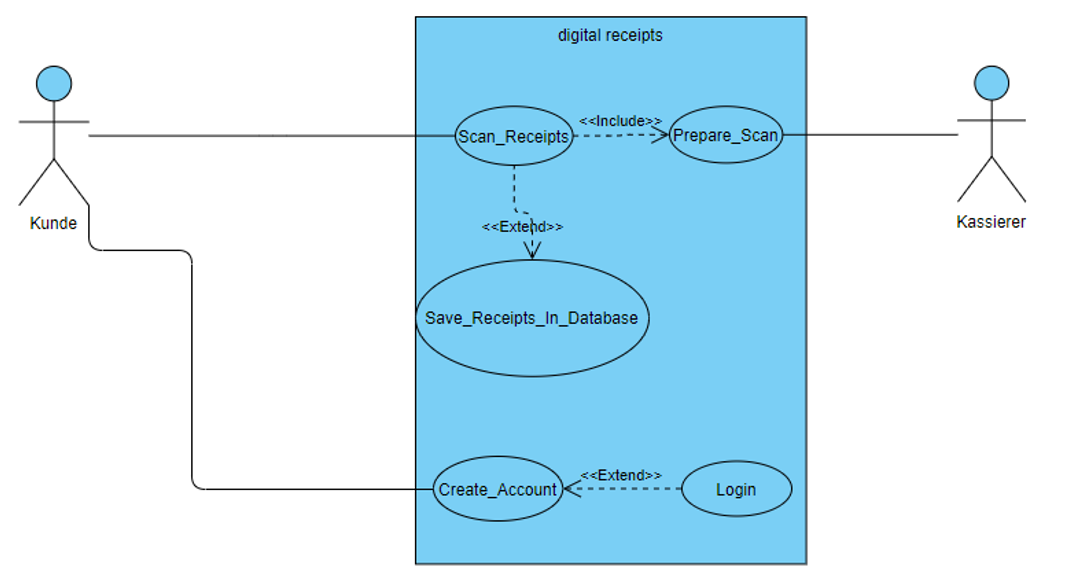
\includegraphics[scale=0.55,keepaspectratio]{"src/u5/UML_Usecase.PNG"}
    \end{enumerate}
    
    
    
\end{enumerate}


% /////////////////////// END DOKUMENT /////////////////////////
\end{document}